\documentclass[tikz,border=4pt]{standalone}
\usepackage{amsmath}
\begin{document}
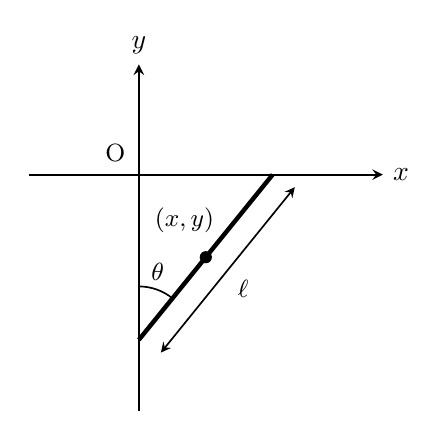
\begin{tikzpicture}[>=stealth, thick, scale=1.0]
  % Axes
  \draw[->, line width=0.7pt] (-1.4, 0) -- (3.1, 0) node[right] {$x$};
  \draw[->, line width=0.7pt] (0, -3.0) -- (0, 1.4) node[above] {$y$};
  \node[above left, font=\small] at (-0.04, 0.04) {$\mathrm{O}$};

  % Rod of length l = 2.7 in 4th quadrant at angle theta = 39 deg from -y axis
  % Top end on +x axis: (2.7*sin(39), 0) = (1.699, 0)
  % Bottom end on -y axis: (0, -2.7*cos(39)) = (0, -2.098)
  \coordinate (T) at (1.699, 0);
  \coordinate (B) at (0, -2.098);
  \coordinate (G) at (0.850, -1.049);

  \draw[line width=1.6pt] (B) -- (T);
  \fill (G) circle (2.2pt);
  \node[font=\small] at (0.58, -0.58) {$(x, y)$};

  % Angle theta at bottom end between +y (along y-axis) and rod
  \draw[line width=0.6pt] (0, -1.42) arc (90:51:0.678);
  \node[font=\small] at (0.24, -1.24) {$\theta$};

  % Length l dimension line parallel to rod (offset to bottom-right)
  \draw[<->, line width=0.6pt] (0.28, -2.26) -- (1.98, -0.16) node[midway, below right, font=\small] {$\ell$};
\end{tikzpicture}
\end{document}
